\documentclass[11pt]{article}
\usepackage[spanish]{babel}
\usepackage[utf8]{inputenc}
\usepackage{geometry}
 \geometry{
 a4paper,
 total={170mm,257mm},
 left=20mm,
 top=20mm,
 }
 \usepackage{graphicx}
 \usepackage{titling}

 \usepackage{fancyhdr}
 \fancypagestyle{plain}{%  the preset of fancyhdr 
     \fancyhf{} % clear all header and footer fields
     \fancyfoot[R]{}
     \fancyfoot[L]{\thedate}
     \fancyhead[L]{Introducción a la Investigación Experimental}
     \fancyhead[R]{\theauthor}
 }
\setlength{\headheight}{13pt}
 \makeatletter
 \def\@maketitle{%
   \newpage
   \null
   \vskip 1em%
   \begin{center}%
   \let \footnote \thanks
     {\LARGE \@title \par}%
     \vskip 1em%
     %{\large \@date}%
   \end{center}%
   \par
   \vskip 1em}
 \makeatother
 
 \usepackage{lipsum}  
 \usepackage{cmbright}

\title{Dependencia de la Temperatura de la Difusión en Tintas Comerciales solubles sobre Agua}
\author{
    \name\\
    {\tt{\email}}}
\date{\today}

\begin{document}
\maketitle
%-----------------------------------------
\begin{abstract}
Este trabajo presenta un estudio experimental sobre la dependencia de la temperatura en el proceso de difusión de tintas comerciales en agua. Se analiza el fenómeno utilizando las leyes de Fick y la teoría de Einstein-Stokes para el movimiento browniano, considerando variables como la concentración, la difusividad y la viscosidad del medio. El experimento se realiza mediante un sistema controlado de termalización y análisis de imágenes para determinar el comportamiento de la difusión en función de la temperatura. Los resultados permitirán verificar las relaciones teóricas y explorar posibles aplicaciones en sistemas más complejos.
\end{abstract}
%-----------------------------------------
\section*{Marco Teórico}
La \textbf{difusión} es el transporte de materia de una parte del sistema a otro parte como resultado de el movimiento aleatorio molecular~\cite{mehrerHistoryBibliographyDiffusion2007} impulsadas a través de la interacción por los gradientes de concentración descritos empíricamente en primer lugar por las \textbf{leyes de Fick}~\cite{fickLiquidDiffusion1995}. La difusión es un fenómeno físico termodinámico gobernado por interacciones mecánico cuánticas atribuidas de la Teoría de Einstein sobre el movimiento browniano~\cite{einsteinUberMolekularkinetischenTheorie1905} que justifican la dinámica molecular o corpuscular de la transferencia de masas, responsable de la mezcla de gases, líquidos y solidos de manera espontanea sin que ocurra un movimiento macroscópico del sistema como lo puede ser la convección, el medio se homogeneizará en un estado donde la densidad de concentración de la sustancia en ese medio tenderá a disminuir en el espacio y el tiempo~\cite{gilExperimentosFisicaUsando2014}.

La primera ley de Fick~\cite{gilExperimentosFisicaUsando2014} relaciona los flujos de partículas por unidad de área $\mathbf{J}$ y los gradientes de concentración $\nabla \mathbf{n}$ en la ec.~\eqref{eq:fick1}:
\begin{equation}
    \mathbf{J} = -D \nabla \mathbf{n},
    \label{eq:fick1}
\end{equation}
donde $\mathbf{n}\equiv n(x,y,z;t)$ es la concentración del soluto, generalmente cantidad en mol o número de partículas por unidad de volumen; $\mathbf{J}\equiv\mathbf{J}(t)$ es el flujo de partículas o moles por unidad de área; y por último $D$ es el coeficiente de \textit{difusividad} que en general dependerá de distintas condiciones  detalladas por la Teoría de Einstein-Stokes.
La segunda ley de Fick es descrita a partir de la ecuación de continuidad del fluido en un elemento infinitesimal de volumen $\Delta V$ que relaciona el flujo del material respecto el tiempo a partir de la ec.~\eqref{eq:fick1.5}
\begin{equation}
    \nabla \mathbf{J} = -\frac{\partial n}{\partial t},
    \label{eq:fick1.5}
\end{equation}
de tal manera que da forma a la \textbf{ecuación de difusión} en la expresión~\eqref{eq:fick2}
\begin{equation}
    \frac{\partial n}{\partial t} = D \nabla^2 n.
    \label{eq:fick2}
\end{equation}

Es esencial destacar la aportación de la Teoría de Einstein-Stokes~\cite{einsteinUberMolekularkinetischenTheorie1905} que relaciona el coeficiente de difusividad $D$ con la temperatura $T$ y el radio de la partícula $r$ en la ec.~\ref{eq:einstein} para la suposición de movimiento browniano en un fluido newtoniano a temperatura constante en un medio isótropo~\cite{leeInkDifussionWater2004}
\begin{equation}
    D = \frac{k_B T}{6 \pi \eta r},
    \label{eq:einstein}
\end{equation}
donde $k_B$ es la constante de Boltzmann, $\eta$ es la viscosidad del medio y $a$ el tamaño de pequeñas esferas en el medio viscoso. La ec.~\eqref{eq:einstein} describe el movimiento browniano de una partícula en un fluido, donde el coeficiente de difusividad $D$ es inversamente proporcional a la viscosidad del medio y directamente proporcional a la temperatura.

Aplicando la ecuación de Fick en el plano bidimensional,
\begin{equation}
    D \left( \frac{\partial^2 C}{\partial r^2} + \frac{1}{r} \frac{\partial C}{\partial r} \right) = \frac{\partial C}{\partial t}
\end{equation}
la solución en cilindricas de la ecuación diferencial parcial~\cite{gilExperimentosFisicaUsando2014} por método de separación de variables bajo condiciones iniciales de $n_0(r=0; t=0) = \delta(0)$ y condiciones de frontera $n(r \to \infty, t) = 0$ queda descrita en la ec.~\eqref{eq:fick2d_sub}\
\begin{equation}
    n(r,t) = \frac{A}{t} \exp{-\frac{r^2}{4Dt}},
    \label{eq:fick2d_sub}
\end{equation}
donde $r$ es el radio euclidiano $r^2 = x^2 + y^2$ sobre las coordenadas del espacio, $t$ es el tiempo y $D$ es el coeficiente de difusividad. Aquí $A$ es una constante arbitraria con relación a $M$ la cantidad de sustancia inicial y total de difusión como
\begin{equation}
    A = \int_{-\infty}^\infty \int_{-\infty}^\infty \mathbf{n} \dd{x}\dd{y} = 4 \pi D M
\end{equation}
luego tenemos la solución final
\begin{equation}
    n(r,t) = \frac{A}{4 D t} \exp{-\frac{r^2}{4Dt}}.
    \label{eq:fick2d}
\end{equation}

Bajo condiciones de frontera más próximas a las condiciones de laboratorio, suponemos una fuente extensa circular de radio $r_0$ en $t=0$ tenemos las condiciones iniciales de cantidad de materia $M$
\begin{subequations}
\begin{align}
    n(r \leq r_0, t=0) = M\\
    n(r > r_0, t=0) = 0
\end{align}
\end{subequations}
obtenemos la solución~\cite{crankMathematicsDiffusion1976} según exp. 
\begin{equation} \label{eq:diffusion2d_round}
    n(r,t) = \frac{M}{2Dt} e^{-\frac{r^2}{4Dt}} \int_{0}^{r_0} e^{-\frac{r'^2}{4Dt}} I_0 \left( \frac{rr'}{2Dt} \right) r' \, dr'
\end{equation}
donde $I_0$ es la función modificada de Bessel de orden cero. Se modelará el problema bajo estos dos primeros principios y estudiaremos que condiciones satisfacen según la oportunidad se de.

Falta notar que podemos considerar únicamente la relación del radio $r$ respecto el tiempo $t$ a través de un frente de onda donde $f$ será la concentración porcentual respecto el total inicial $n_0$ elegido según convenga para determinar con el radio la expresión
\begin{equation}
    f = \exp{-(x^2_0/4Dt)} \to x_0^2 = 4 \tau \ln(1/f)
\end{equation}
con lo que podemos llamar $\tau$ tiempo reducido.

Es esencial en cualquier problema práctico tener en cuenta las contribuciones a la disolución debidas a las corrientes de convección~\cite{Cussler_2009} que corren de forma ortogonal \ref{fig:dif_vs_conv}, se requiere por tanto de evitar los gradientes de temperatura $\nabla T$ ajustando el esquema experimental a proporcionar un sistema termodinámico aislado: a través de un baño térmico, evitar evaporación, disminuir el volumen para solventar evitar las corrientes. 
\begin{figure}[htp]
    \centering
    


\tikzset{every picture/.style={line width=0.75pt}} %set default line width to 0.75pt        

\begin{tikzpicture}[x=0.75pt,y=0.75pt,yscale=-1,xscale=1]
%uncomment if require: \path (0,300); %set diagram left start at 0, and has height of 300

%Shape: Rectangle [id:dp10359013539871109] 
\draw   (112.67,59.67) -- (147.42,59.67) -- (147.42,94.06) -- (112.67,94.06) -- cycle ;
%Straight Lines [id:da5541892841157354] 
\draw    (148.75,76.06) -- (181.42,76.06) ;
\draw [shift={(183.42,76.06)}, rotate = 180] [color={rgb, 255:red, 0; green, 0; blue, 0 }  ][line width=0.75]    (10.93,-3.29) .. controls (6.95,-1.4) and (3.31,-0.3) .. (0,0) .. controls (3.31,0.3) and (6.95,1.4) .. (10.93,3.29)   ;
%Straight Lines [id:da37648765041965193] 
\draw    (129.42,94.06) -- (129.42,120.06) ;
\draw [shift={(129.42,122.06)}, rotate = 270] [color={rgb, 255:red, 0; green, 0; blue, 0 }  ][line width=0.75]    (10.93,-3.29) .. controls (6.95,-1.4) and (3.31,-0.3) .. (0,0) .. controls (3.31,0.3) and (6.95,1.4) .. (10.93,3.29)   ;

% Text Node
\draw (82.67,69.07) node [anchor=north west][inner sep=0.75pt]    {$\Delta y$};
% Text Node
\draw (115.33,35.73) node [anchor=north west][inner sep=0.75pt]    {$\Delta r$};
% Text Node
\draw (122,132) node [anchor=north west][inner sep=0.75pt]   [align=left] {Convección};
% Text Node
\draw (195.33,67.33) node [anchor=north west][inner sep=0.75pt]   [align=left] {Difusión};


\end{tikzpicture}
    \caption{Comparación entre difusión pura y difusión convección.}
    \label{fig:dif_vs_conv}
\end{figure}
%-----------------------------------------
\section*{Marco Experimental}
El arreglo experimental se basa principalmente en el proyecto 190 del Cap. 57 de Salvador Gil~\cite{gilExperimentosFisicaUsando2014} con el esquema propuesto como en la fig.~\ref{fig:esquema_experimental}. Esta es una guía experimental y no se tienen resultados de consulta al respecto, pero se obtiene el comportamiento de la concentración $\mathbf{n(r)}$ respecto el tiempo reducido en la fig.~\ref{fig:Arr1_n_vs_r}
\begin{figure}[htp]
    \centering
    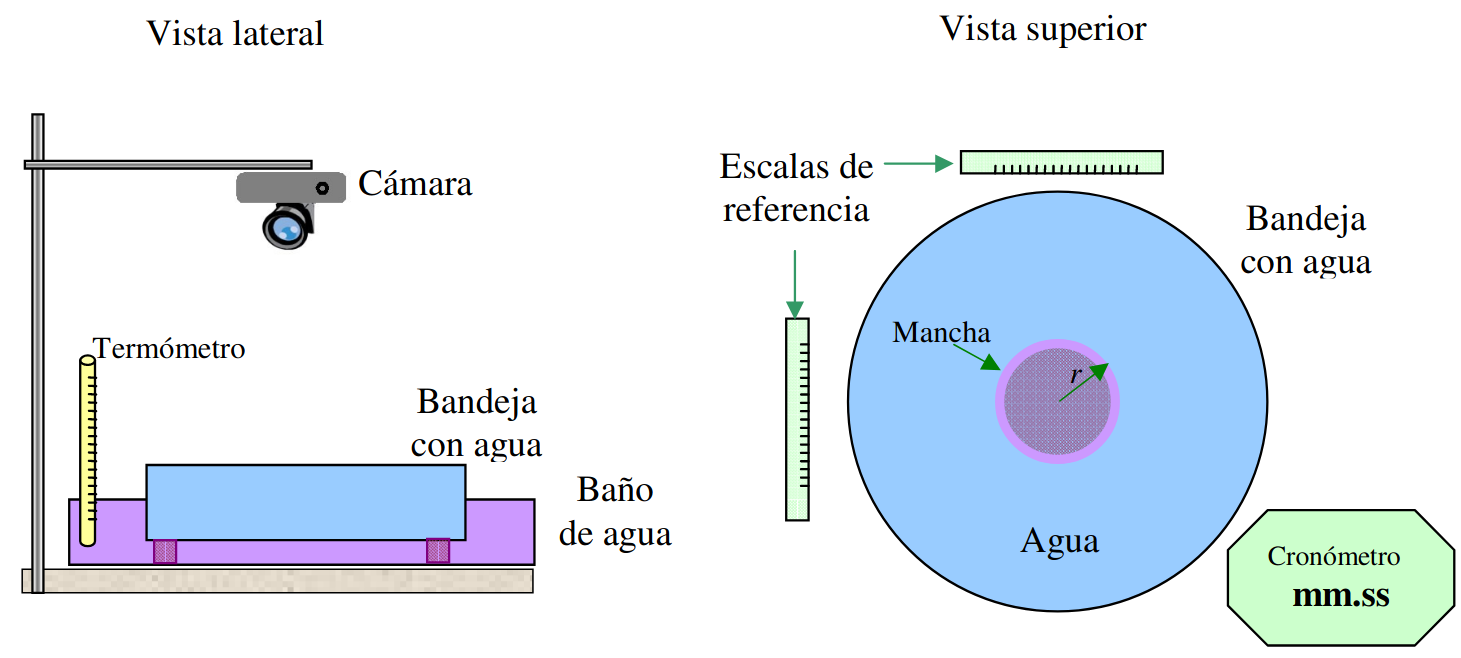
\includegraphics[width=0.8\textwidth]{figs/esquema_refGil.png}
\caption{Esquema del experimento de difusión en dos dimensiones. Tomado de~\cite{gilExperimentosFisicaUsando2014}.}\label{fig:esquema_experimental}
\end{figure}
\begin{figure}[htp]
    \centering
    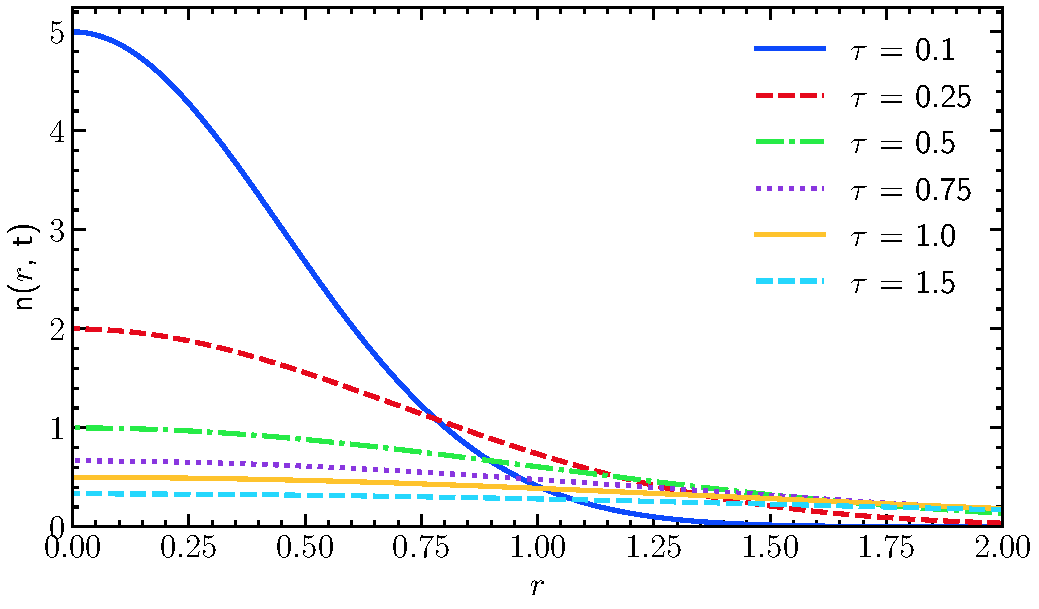
\includegraphics[width=0.8\textwidth]{figs/n(r,t)_vs_r.pdf}
    \caption{Perfil de concentración $n$ respecto el radio según para una variedad de tiempos reducidos $\tau$ esperados. Se observa que para $\tau\to 0$ resulta ser $n_0 = \delta(0)$. Basado de~\cite{gilExperimentosFisicaUsando2014}.}
    \label{fig:Arr1_n_vs_r}
\end{figure}
Se dispone un recipiente de vidrio con agua sobre un baño térmico a una temperatura $T_a$, se propone regular la temperatura con hielo y agua caliente, se propone también utilizar una resistencia $R$. Las escalas de referencia en vertical y horizontal como reglas milimetradas ($\Delta r = \pm 0.1 cm$), aunque también se puede disponer de una grilla como un papel milimetrado. Se utilizará un cronómetro de referencia ($\Delta t = \pm 0.1 \, \unit{\second}$) que será leído por la cámara posicionada en un soporte en posición cenital al fenómeno, se utilizará un cuentagotas con tinta (de estampar \textit{stamp}) puesta en el punto central del recipiente y si es posible para líquido-líquido.

Las condiciones supuestas para el arreglo experimental son: sin convección debido al grosor $\Delta y= 1 \, \unit{\centi\meter}$; reducida interacción con el aire circundante, se propone aislante transparente; baño termostatado, con variaciones de temperatura menores a $\Delta T = \pm 1 \, \unit{\celsius}$; bandeja de vidrio con el fin de obtener el perfil de luminancia $L$ asumiendo $L \propto \mathbf{n}$; y con una concentración inicial mínima.

Se estudió también el arreglo experimental realizado por Bianchi et.al.~\cite{micaelaDifusionKMnO4Agua2006} propuesto para la solución bidimensional con radio inicial $r_0$. En el esquema propuesto~\ref{fig:esquema_bianchi} añaden el uso del computador para visualización de imagen, pero se elimina el baño térmico.
\begin{figure}[htp]
    \centering
    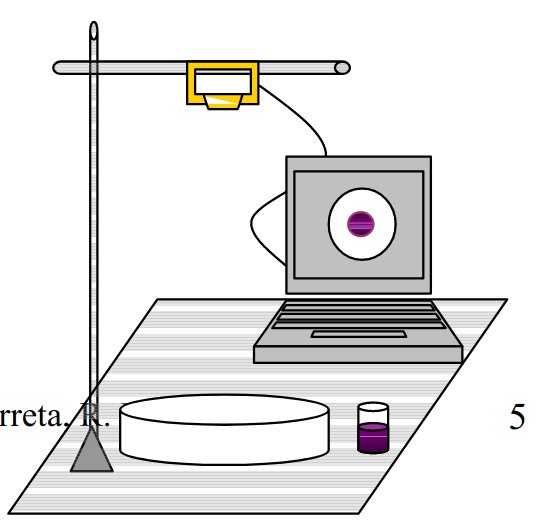
\includegraphics[width=0.35\textwidth]{figs/esquema_Bianchi.png}
    \caption{Esquema experimental propuesto por Bianchi et al. Tomado de~\cite{micaelaDifusionKMnO4Agua2006}.}
    \label{fig:esquema_bianchi}
\end{figure}
\begin{figure}[htp]
    \centering
    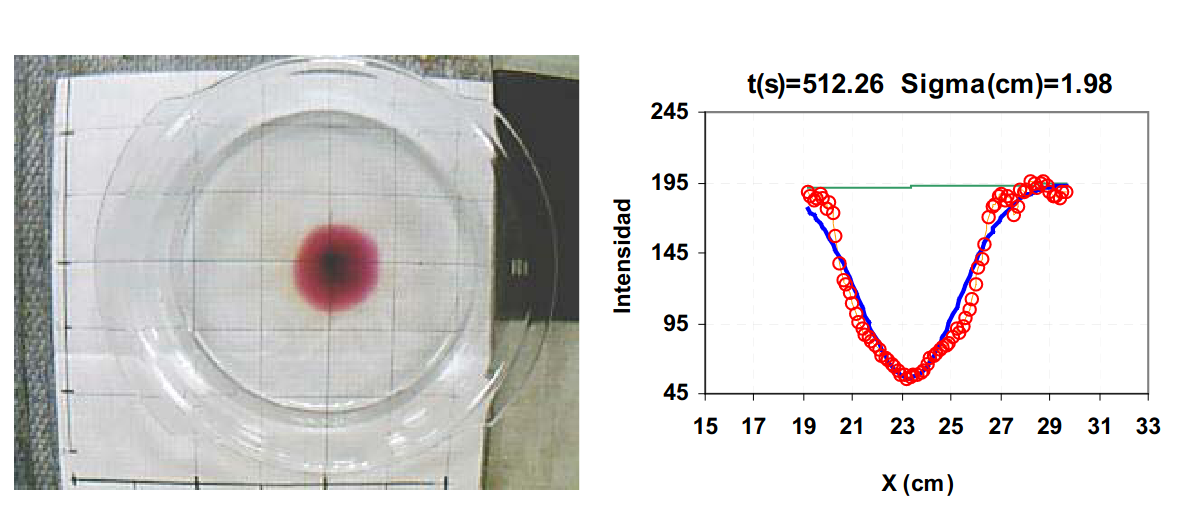
\includegraphics[width=0.85\textwidth]{figs/arrBianchi_fotos.png}
    \caption{Mediciones del arreglo experimental propuesto por Bianchi et al. Tomado de~\cite{micaelaDifusionKMnO4Agua2006}. }
    \label{fig:fotos_bianchi}
\end{figure}
Se destaca el uso adecuado del perfil de medición a través de software del ajuste gaussiano esperado el esquema resuelto. Los datos comprendidos, por lo que se espera implementar un proceso similar. Resolviendo con los datos obtenidos el factor de difusión $D$~\ref{fig:bianchi_plot_D}. Las mediciones respecto variación de temperatura y la dependencia temporal del radio difusivo también resultan insatisfactorias según el ajuste propuesto por este artículo, por lo que se destaca únicamente la técnica de software.
\begin{figure}[H]
    \centering
    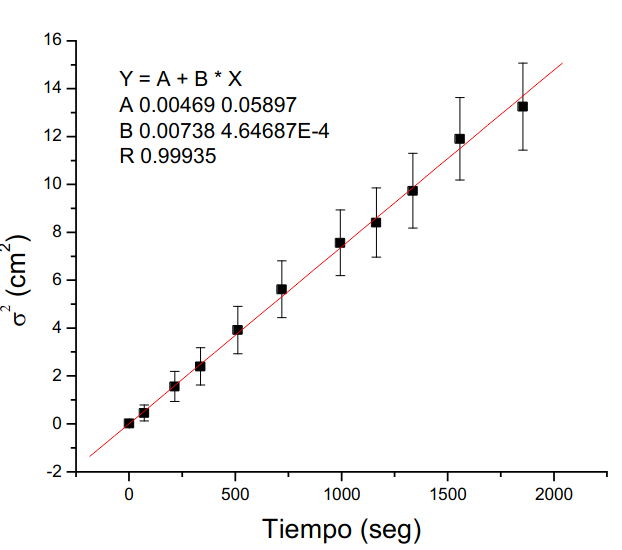
\includegraphics[width=0.6\textwidth]{figs/arrBianchi_plotGaussiano.png}
    \caption{Determinación del factor de Difusión $D$. Tomado de~\cite{micaelaDifusionKMnO4Agua2006}. }
    \label{fig:bianchi_plot_D}
\end{figure}

En este sentido, es fundamental destacar el artículo de Lee et al.~\cite{leeInkDifussionWater2004} sobre la difusión del agua utilizando nuevamente la aproximación del radio inicial como un circulo de radio $r_0$. En esta oportunidad, a partir de técnicas químicas se puede determinar previamente la viscosidad $\eta$ y la densidad $\rho$ de las tintas utilizadas: tinta de estampar (\textit{stamp}) y tinta \textit{Quink ink blue} de la compañia Parker, obteniendo apreciaciones precisas sobre el cambio de estos parámetros respecto diferentes temperaturas. La toma de datos se basa en un montaje principal y ya descrito antes, se exhiben las fotos tomadas en fig.~\ref{fig:arrLee_fotos}.
\begin{figure}[htp]
    \centering
    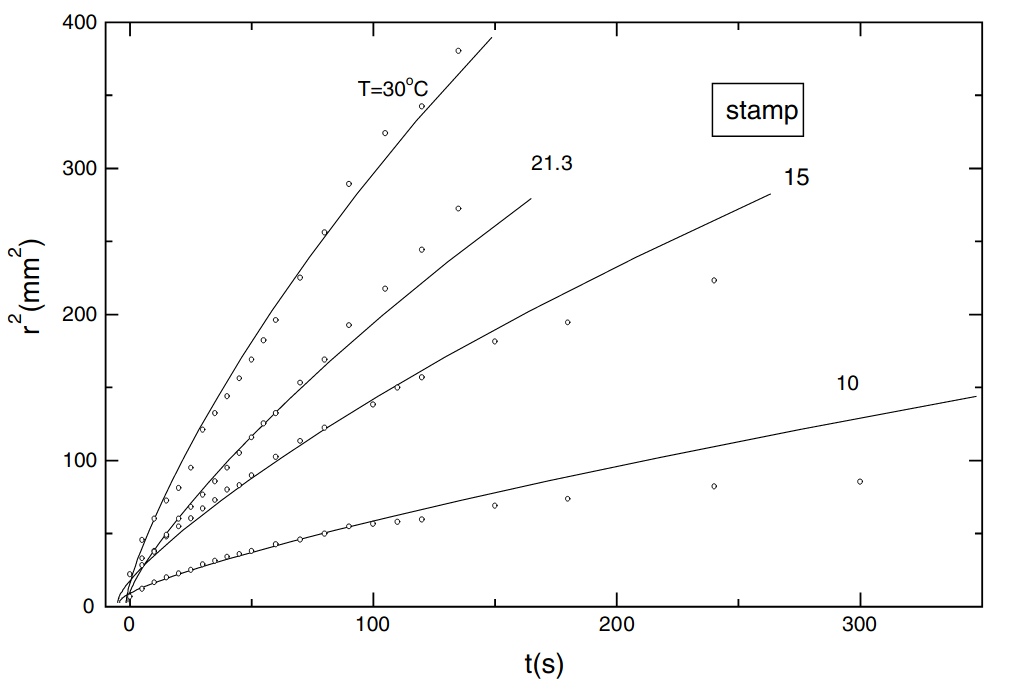
\includegraphics[width=0.7\textwidth]{figs/arrLee_plotStamp.png}
    \caption{Dependencia de la variación del radio $r$ respecto el tiempo transcurrido $t$ para diferentes temperaturas $T_i$ para tinta de estampar. Tomado de \cite{leeInkDifussionWater2004}.}
    \label{fig:arrLee_plot_stamp}
\end{figure}

Apreciaremos únicamente el estudio de la tinta \textit{stamp} y tomaremos en cuenta las restricciones comentadas en el artículo: utilizar únicamente tinta a base de agua; para una completa apreciación de la variación de viscosidad se tomarán medidas con un \textit{tubo Ubbelohde} y las densidades con una balanza; tomar el grosor del agua a 1 cm para determinar solamente el fenómeno difusivo; centrarse en el radio $r$ para determinar posteriormente la energía de activación por medio de la \textbf{ecuación de Arrhenius}, donde obtienen la conclusión del estudio a través de la fig.~\ref{fig:arrLee_plot_energia}, los resultados son posiblemente comparables con el esquema que se prevee.
\begin{figure}[htp]
    \centering
    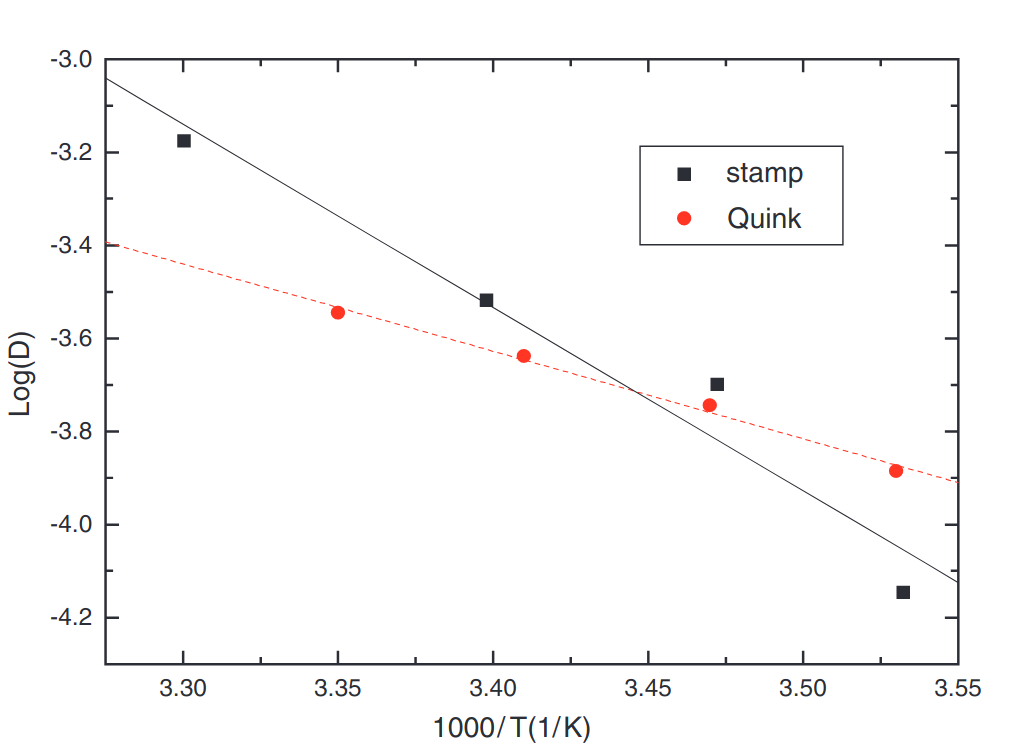
\includegraphics[width=0.7\textwidth]{figs/arrLee_energia_activacion.png}
    \caption{Dependencia del factor de difusividad respecto la temperatura en comparación con la tinta Quink blue ink y la tinta \textit{stamp}.}
    \label{fig:arrLee_plot_energia}
\end{figure}
\begin{figure}[htp]
    \centering
    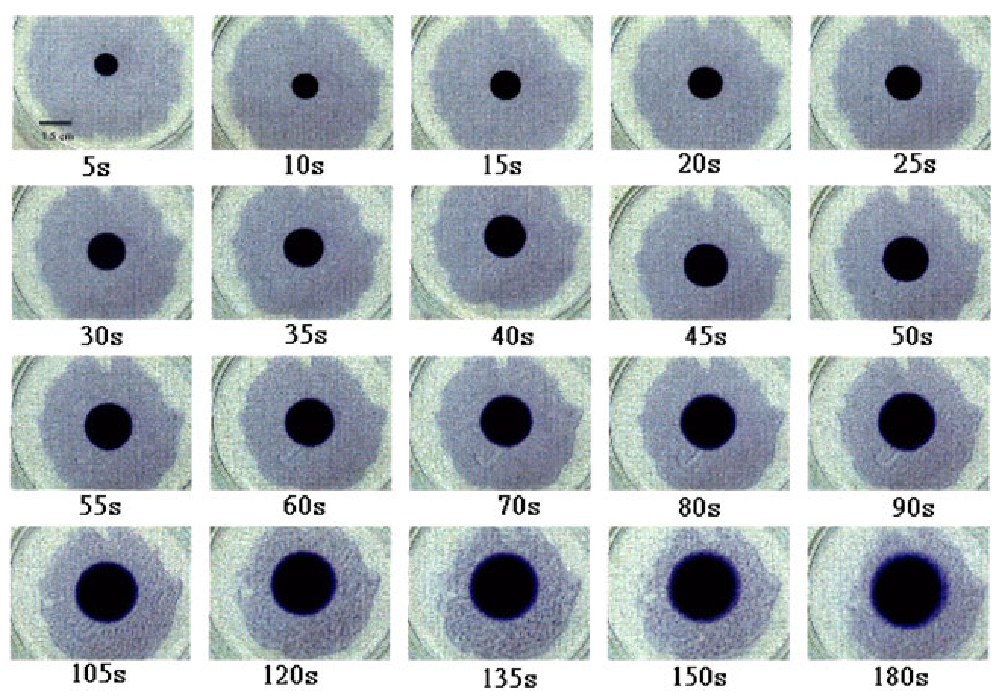
\includegraphics[width=0.7\textwidth]{figs/arrLee_fotos.png}
    \caption{Toma de datos a partir de una luminosidad apreciable del radio $r$ a partir de imagenes consecutivas. Tomado de~\cite{leeInkDifussionWater2004}.}
    \label{fig:arrLee_fotos}
\end{figure}

La última referencia principal que se utilizará en este estudio es respecto al montaje de \textbf{Nir Livne} sobre el error principal común acerca de estos esquemas y cómo genera un esquema para aislar los fenómenos convectivos de la práctica experimental. En este experimento se utiliza una pipeta cilindrica pequeña para estudiar la difusividad unidimensional en la fig.~\ref{fig:arrNir_fotos}, se toman los datos a través de perfiles de luminancia y se analiza factor de densidad $f$ dado a través del cuál se determina la relación difusividad temporal sobre el radio en la fig.~\ref{fig:arrNir_plot}.

Aquí se destaca el uso del software, el cuidado de eliminar los términos de convección con el aislamiento térmico del cuál se prevee se pueda replicar y se toma en cuenta los tiempos que determina la teoría~\cite{leeInkDifussionWater2004,nirlRealDiffusionExperiment} para conocer la viabilidad de la aplicación del experimento en laboratorio.

\begin{figure}[htp]
    \centering
    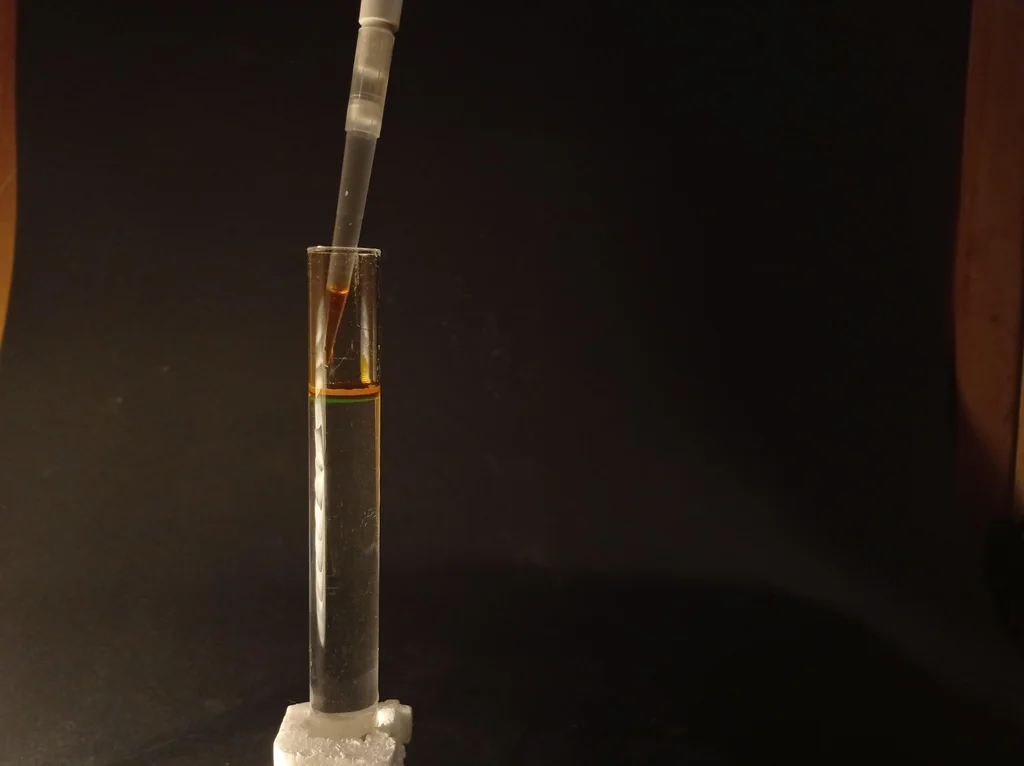
\includegraphics[width=0.5\textwidth]{figs/arrNir_esquema.png}
    \caption{Esquema experimental y toma de datos de la difusión unidimensional. Tomado de~\cite{nirlRealDiffusionExperiment}.}
    \label{fig:arrNir_fotos}
\end{figure}
\begin{figure}[htp]
    \centering
    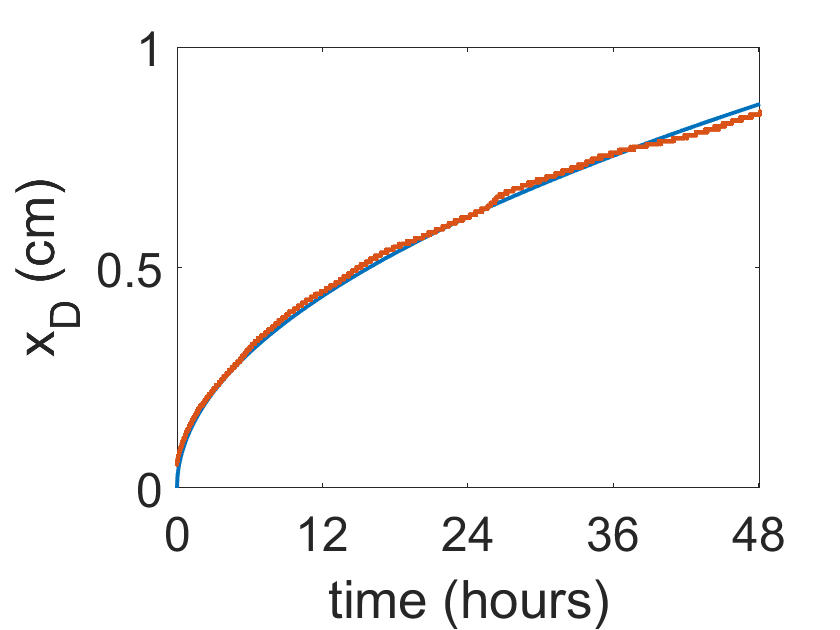
\includegraphics[width=0.7\textwidth]{figs/arrNir_plot.png}
    \caption{Resultado experimental de la difusividad $D$ de $4 \times 10^-6 \, \unit{cm^2/\second}$. Tomado de~\cite{nirlRealDiffusionExperiment}.}
    \label{fig:arrNir_plot}
\end{figure}

Por último, se destaca que debido a a que las referencias sobre gas-gas~\cite{hanTemperatureDependenceOxygen1996} requiere métodos sofisticados fuera del alcance experimental actual; solido-líquido~\cite{micaelaDifusionKMnO4Agua2006} requiere permanganato de potasio que no se consiguió y el costo ya es elevado, además que en otros solidos también es requerido técnicas sofisticadas; líquido-sólido~\cite{silvaDispersionInkPapers2008a} no presentaba esquema experimental y no existían suficientes fuentes para poder tener un esquema completo. También se destacan las formas avanzadas de difusión descritas por la aproximación de fractal~\cite{heFractalApproachDiffusion2022} que requiere técnicas matemáticas más avanzadas.

%-.-.-.-.-.-.-.-.-.-.-.-.-.-.-.-.-.-.-.-.-.-.-.-.-.-.-.-.
\subsection*{Propuesta Experimental}
A lo largo de la sección previa se fueron denotando los aspectos para los cuales el primer arreglo experimental fuera modificado en orden a las restricciones y condiciones para la realización del experimento. Se presenta entonces un esquema de Gil~\ref{fig:esquema_experimental} con las siguientes modificaciónes:
\begin{enumerate}
    \item Se presentará mayor aislamiento térmico, aplicando un recubrimiento sobre la base principal, evitando contacto térmico con el baño y evitando fuentes de ruido que incurran en una apreciable deshomogeneidad en la práctica. También fuera de fuente solar, en sombra a una temperatura constante
    \item Se establece a partir de Bianchi et al.~\cite{micaelaDifusionKMnO4Agua2006} la posibilidad de tomar perfiles de luminancia, para lo cual se plantea una base de vidrio sobre el baño térmico de color blanco, de tal manera que se pueda aplicar suficiente luz. Aquí se propone una fuente lumínica cenital y una inferior en una línea para tomar el perfil de manera uniforme.
    \item Se estandariza el uso del gotero de tal manera que sea posible tomar las mediciones con un $M\sim cte$ para cada práctica.
    \item Se utilizará como tintas las siguientes: tinta \textit{stamp}~\cite{leeInkDifussionWater2004}, azul de metileno~\cite{selifonovDeterminationDiffusionCoefficient2019} y tinta china, por lo que la práctica será únicamente líquido-líquido.
    \item Se integrará a la medición directa el computador con conexión con la cámara, para determinar directamente las posibilidades del experimento.
    \item Se integrará el uso de la resistencia térmica en el baño, permitirá controlar la temperatura de manera más eficiente que solo con agua caliente, aunque no se descarta.
\end{enumerate}

Las variables sistemáticas   son las siguientes, teniendo en cuenta que aquella con ( serán sistemáticas:
\begin{itemize}
    \item \textbf{Temperatura del Baño} $T_b$ (K): Se espera que la temperatura del agua pueda variarse y termalizarse con la temperatura real $T$ del recipiente, que se pueda variar entre $T_b = 10 \pm 1 \, \unit{\degreeCelsius}$ y $T_b = 70 \pm 1 \, \unit{\degreeCelsius}$ para evitar perturbaciones por evaporación u otros. Se espera tener curvas diferentes curvas de difusión para cada temperatura y posterior hacer el análisis en el rango lineal~\cite{leeInkDifussionWater2004}.
    \item \textbf{Tiempo} $t$ (s): Se espera medir rangos de tiempo suficientemente largos para verificar el fenómeno completo basado en $\tau\equiv Dt$ tiempos de difusión con cronómetro. Se tienen también curvas de $\tau$ respecto cada $n$ vs $t$~\cite{leeInkDifussionWater2004}.
    \item \textbf{Cantidad} $m$ (gr): Se espera que la cantidad de tinta sea controlada por el cuentagotas que tendrá determinado un peso a partir de la densidad de la tinta $\rho_0$ o medición directa. Se determinará posteriormente la posibilidad de esta variación.

Las variables principales que determinar son:
\begin{itemize}
    \item \textbf{Radio} $\mathbf{r}$ (cm): El radio de difusión será medido a partir de las imágenes obtenidas del experimento, utilizando software de análisis de imágenes.
    \item \textbf{Concentración} $\mathbf{n}$ (mol/cm$^3$): se utilizará el perfil de luminancia para poder determinar la concentración. Para ello se varia 
    \item \textbf{Difusividad} $\mathbf{D}$ (m$^2$/s): Se espera que el coeficiente de difusividad de la tinta en agua sea determinado por las condiciones según ec.~\ref{eq:einstein}, aunque hay una derivación teórica utilizando la energía de activación química~\cite{leeInkDifussionWater2004}.
    \item \textbf{Viscosidad} $\mathbf{\eta}$ ($\unit{\pascal} \cdot \unit{\second}$): Podremos controlar parcialmente la viscosidad de la tinta según la viscosidad inicial (¿determinada por fabricante?).
\end{itemize}

\end{itemize}
%-----------------------------------------
\section*{Materiales}
Los materiales que se utilizarán son:
\begin{itemize}
    \item \textbf{Cámara}: Cámara de dispositivo movil Nokia G21 con sensor JN1 de 50MP.
    \item \textbf{Soporte}: Estable y ajustable en tres grados de libertad, se colocará la cámara de forma cenital sobre este junto con el foco.
    \item \textbf{Iluminación}: Luz LED para la base y bombillo led para la vista superior, se tantea la utilidad según convenga. Requieren fuente de 12 V.
    \item \textbf{Recipiente Principal}: Recipiente de vidrio circular de 25 cm de diametro.
    \item \textbf{Recipiente Baño}: Recipiente aislante térmico, plástico transparente.
    \item \textbf{Agua normal}: Agua de llave, el agua destilada era muy cara y no hay referencia explicita que tenga esta restricción.
    \item \textbf{Resistencia Térmica}: Resistencia de cerámica capaz de calentar el agua a temperaturas hasta 40°C y posiblemente más de manera estable.
    \item \textbf{Termómetro}: Termómetro de precisión, se tomará prestado en el laboratorio.
    \item\textbf{Cronómetro}: Cronómetro digital de precisión para comparar con el video o gestionar las fotos.
    \item\textbf{Reglas}: Reglas milimetradas o papel milimetrado para establecer la escala de referencia.
    \item\textbf{Tintas}: Tinta china, tinta de estampado, tinta de azul de metileno.
    \item \textbf{Cuentagotas}: Para determinar medidas más precisas de la cantidad de sustancia inicial.
\end{itemize}

\section*{Secuencia de Experimentos}
Basado en lo anterior, la práctica se realizará de la siguiente manera

\begin{enumerate}
    \item \textbf{Determinación del perfil de difusión en condiciones estándar:} 
    Se realizará el experimento inicial utilizando tinta \textit{stamp} en agua a temperatura ambiente $T_a$. Se pretende estudiar el perfil de concentración $n(r,t)$ respecto al radio $r$ y el tiempo $t$, verificando la solución teórica de la ecuación de difusión en dos dimensiones. 
    
    Esto dará claridad de la viabilidad de las fotos, del tiempo medio del experimento, de por ahora no complicarse con las condiciones de variación de temperatura.

    \item \textbf{Estudio de la difusión para diferentes tintas:} 
    Se realizarán experimentos utilizando diferentes tintas (tinta \textit{stamp}, azul de metileno y tinta china) para analizar cómo las propiedades químicas y físicas de las tintas afectan el perfil de difusión y el coeficiente de difusión $D$, si es apreciable la diferencia de estas difusiones en un orden no mayor a varias horas de tiempo (recuerdese~\cite{nirlRealDiffusionExperiment}).


    \item \textbf{Análisis de las imagenes tomadas a través de \texttt{tracker}:} 
    Se tomará el perfil de luminancia $L$ de las imágenes obtenidas durante los experimentos y se verificará si $L \propto n(r,t)$, utilizando software de análisis de imágenes.

    \item \textbf{Estudio de la dependencia de la difusión con la temperatura:} 
    Se repetirá el experimento variando la temperatura del baño térmico en un rango de $10 \, \unit{\degreeCelsius}$ a $70 \, \unit{\degreeCelsius}$. Se pretende analizar cómo el coeficiente de difusividad $D$ depende de la temperatura, verificando la relación teórica dada por la ecuación de Einstein-Stokes o de la ecuación de Arrhenius.

    \item \textbf{Determinación de la energía de activación:} 
    A partir de los datos obtenidos en el experimento de variación de temperatura, se calculará la energía de activación del proceso de difusión utilizando la ecuación de Arrhenius.

    \item \textbf{Estudio del efecto de la viscosidad:} 
    Se medirá la viscosidad $\eta$ de las tintas utilizando un tubo de Ubbelohde y se analizará su influencia en el coeficiente de difusión $D$, verificando la relación teórica de Einstein-Stokes.

\end{enumerate}

\section*{Recomendación AI}
Se consultará a la inteligencia artificial acerca de posibles experimentos complementarios o añadidos en este proceso:

\begin{tcolorbox}[colback=blue!5!white,colframe=blue!75!black,title=Propuesta de Experimento Complementario]
Con el fin de enriquecer el análisis del fenómeno de difusión de tinta en agua y su relación con medidas estadísticas como la media, se propone un experimento complementario que permita observar cómo varía la difusión en función de la temperatura del agua o del tipo de tinta utilizada.

\subsection*{Nombre del experimento}
Comparación del radio medio de difusión en función de la temperatura del agua o del tipo de tinta.

\subsection*{Objetivo}
Investigar cómo influyen la temperatura del agua o el tipo de tinta en la velocidad de difusión, utilizando como medida cuantitativa el \emph{radio medio} de la mancha formada a lo largo del tiempo.

\subsection*{Procedimiento}
\begin{enumerate}
    \item Preparar una bandeja con agua a temperatura ambiente. Registrar la temperatura inicial con un termómetro.
    \item Colocar una gota de tinta en el centro de la superficie del agua y comenzar a registrar el proceso con una cámara cenital.
    \item Repetir el procedimiento para diferentes temperaturas del agua (por ejemplo, agua fría a $10\,^\circ$C y agua caliente a $40\,^\circ$C), o con distintos tipos de tinta (negra, azul, roja).
    \item Extraer fotogramas del video en intervalos regulares de tiempo.
    \item En cada fotograma, medir el radio de la mancha en varias direcciones desde el centro, y calcular el \textbf{radio medio} $\bar{r}(t)$ como el promedio de dichas medidas.
    \item Comparar gráficamente las curvas $\bar{r}(t)$ para las distintas condiciones experimentales.
\end{enumerate}

\subsection*{Relación con el análisis de medias}
Este experimento permite extender el uso de la media como herramienta para describir la evolución de un sistema físico. Al calcular el radio medio de la mancha de tinta, se obtiene una medida central que representa el crecimiento global del área afectada por la difusión. Además, al comparar distintos escenarios, se puede analizar cómo la media varía en respuesta a cambios en variables físicas como la temperatura o la composición del fluido.
\end{tcolorbox}



%-----------------------------------------

\bibliographystyle{IEEEtran}
\bibliography{references}
\end{document}
